\documentclass[8pt,a4paper,landscape]{scrartcl} 
\usepackage[left=1cm,right=1cm,top=1cm,bottom=1cm,landscape]{geometry} 
\usepackage[utf8]{inputenc} 
\usepackage[ngerman]{babel} 
\usepackage{multicol} 
\usepackage{lipsum}
\usepackage{amsmath} 
\usepackage{amsfonts} 
\usepackage{amssymb} 
\usepackage{gensymb} 
\usepackage{dsfont} 
\usepackage{calc} 
\usepackage{tabularx}
\usepackage[table]{xcolor}
\usepackage{arydshln}
\usepackage{tikz}
\usepackage{multirow}
\usepackage{mathtools}
\usetikzlibrary{calc,arrows}
%\usepackage[permil]{overpic} \usepackage{graphicx} \graphicspath{{gfx/}} 

\definecolor{Gray}{gray}{0.9}
\definecolor{LightCyan}{rgb}{0.88,1,1}


\newcolumntype{Y}{>{\centering\arraybackslash}X}
\renewcommand\tabularxcolumn[1]{m{#1}}% for vertical centering text in X column
\renewcommand{\arraystretch}{1.25}
\renewcommand{\arraycolsep}{1.25pt}
\newcommand{\tikzmark}[1]{%
	\tikz[overlay,remember picture] \node (#1) {};}


\author{Levin Baumann} 



\title{Formelsammlung Sensorik} 

\begin{document} 
\setlength{\columnsep}{1cm} 
\begin{multicols*}{3}

\subsection*{Farbräume}
$ R,G,B = [255, 255, 255] \text{\hspace{1.5cm}1 Byte pro Farbe}$

\subsubsection*{RGB in HSI Umrechnung}
\noindent
Falls $ R = G = B $, dann $ H $ undefiniert.\\
Falls $ R = G = B = 0 $, dann $ S $ undefiniert.
\begin{alignat*}{1}
	c &= \arccos\left(\dfrac{2R-G-B}{2\sqrt{(R-G)^2+(R-B)(G-B)}}\right)\\
	H &= \Bigg\{ \begin{matrix*}
			c & \text{falls } B<G\\
			360-c & \text{sonst}
		\end{matrix*}\\
	S &= 1 - \dfrac{3}{R+G+B}\cdot[\text{min}(R,G,B)]\\
	I &= \dfrac{1}{3}(R+G+B)\\
\end{alignat*}

\subsubsection*{RGB24 nach 8bit Graustufen}
$ g = (R + G + B) / 3 $\\
oder\\
$ g = 0.299\cdot R + 0.587\cdot G + 0.114\cdot B $\\

\subsubsection*{Prewitt-Filter}
$
p_x = \left[\begin{Array}{ccc}
	-1 & 0 & 1\\
	-1 & 0 & 1\\
	-1 & 0 & 1\\
\end{Array}\right]
$
\hspace{1cm}
$
P_x = \dfrac{\delta g(x,y)}{\delta x}
$
\hspace{1cm}
$ M \approx \sqrt{P_x^2 + P_y^2} $

$
p_y = \left[\begin{Array}{ccc}
	-1 & -1 & -1\\
	0 & 0 & 0\\
	1 & 1 & 1\\
\end{Array}\right]
$
\hspace{1cm}
$ p_y = \dfrac{\delta g(x,y)}{\delta y} $


\subsubsection*{Gauß-/Mittelwert-Filter}

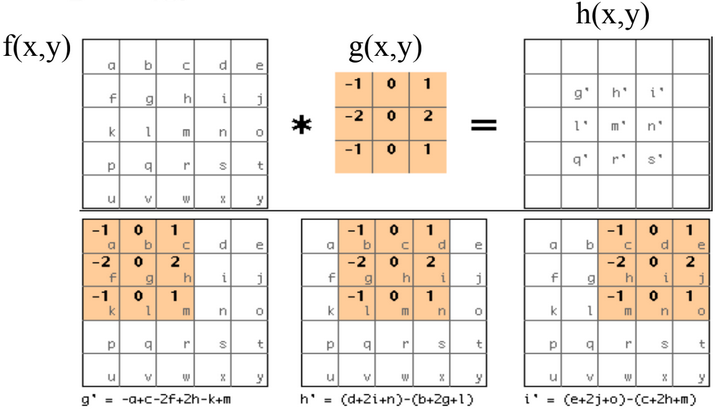
\includegraphics[width=\columnwidth]{Gauss}
Bei Mittelwert: $ 3\times 3 $ Matrix mit allen Werten $ 1 $. Anschließende Division durch $ 9 $.
\subsubsection*{Sobel-Filter}
$
S_x = \left[\begin{Array}{ccc}
	-1 & 0 & 1\\
	-2 & 0 & 2\\
	-1 & 0 & 1\\
\end{Array}\right]
$
\hspace{1cm}
$
S_x = \dfrac{\delta g(x,y)}{\delta x}
$
\hspace{1cm}
$ M \approx \sqrt{S_x^2 + S_y^2} $

$
S_y = \left[\begin{Array}{ccc}
	-1 & -2 & -1\\
	0 & 0 & 0\\
	1 & 2 & 1\\
\end{Array}\right]
$
\hspace{1cm}
$ S_y = \dfrac{\delta g(x,y)}{\delta y} $
\subsubsection*{Roberts-Filter}
$ R_x=\left(\begin{Array}{cc}
	-1 & 0\\
	0 & 1
\end{Array}\right), R_y=\left(\begin{Array}{cc}
0 & -1\\
1 & 0
\end{Array}\right)$\\
$R(g(x,y)) = |R_x(g(x,y))|+|R_y(g(x,y))| $
\subsubsection*{Laplace-Filter}
$ \nabla^2 \approx \left(\begin{Array}{ccc}
	0 & 1 & 0\\
	1 & -4 & 1\\
	0 & 1 & 0\\
\end{Array}\right), \nabla^2g(x,y) = \dfrac{\delta^2g(x,y)}{\delta x^2} + \dfrac{\delta^2g(x,y)}{\delta y^2}$
\subsection*{Projektion}
Projektion eines Szenepunktes $ P=(X,Y,Z) $ auf Bildpunkt $ p=(u,v,w) $ mit Brennweite $ f $:
$
\dfrac{-u}{f} = \dfrac{X}{Z}, \hspace{.1cm} \dfrac{-v}{f} = \dfrac{Y}{Z}, \hspace{.1cm} w = -f 
$\\
Rückprojektion: $ X = -\dfrac{uZ}{f}, \hspace{.1cm} Y=-\dfrac{vZ}{f}$\\
Perspektivprojektion: \\
$ p= \left(\begin{Array}{c}
	u \\ v \\ w
\end{Array}\right) = \left(\begin{Array}{c}
u \\ v \\ -f
\end{Array}\right) = -\dfrac{f}{Z}\left(\begin{Array}{c}
X \\ Y \\ Z
\end{Array}\right) = -\dfrac{f}{Z}P$

\subsubsection*{Linsensysteme}
$ \dfrac{1}{Z} + \dfrac{1}{Z'} = \dfrac{1}{f} $\\
$ \dfrac{1}{Z} + \dfrac{1}{Z'} \approx \dfrac{1}{Z'} \Rightarrow \dfrac{1}{Z'} \approx \dfrac{1}{f}$\\
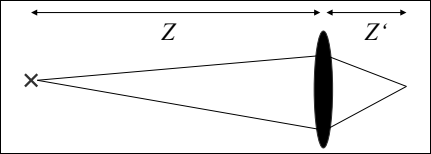
\includegraphics[width=\columnwidth]{Linsensysteme}

\subsubsection*{Iterative Endpoint Fit}
Gegeben: Punkte $ P $, Linien $ L={} $, Distand $ d $\\
\begin{itemize}
	\setlength{\itemsep}{1pt}
	\setlength{\parskip}{0pt}
	\setlength{\parsep}{0pt}
	\item Finde $ x_1, x_2 \in P $ mit $ ||x_1-x_2||=max $; verbinde sie durch Linie $ l_0=\{X_1, X_2\}, L = L\cup \{l_0\} $
	\item Für alle $ l \in L $:
	\subitem Finde $ x \in P $ mit $ ||l-x||=max $
	\subitem Wenn $ ||l-x|| < d $:
	\subsubitem Ordne $ x $ als Mitgliedspunkt $ l $ zu
	\subsubitem Entferne $ x $ aus $ P $
	\subitem Sonst:
	\subsubitem Brich $ l $ in $ l_1 = \{x_y,x\} $ und $ l_2=\{x,x_2\} $ auf
	\subsubitem Alle Mitgliedspunkte von $ l $ wieder in $ P $\\
	\subitem $ P $ leer $ \rightarrow $ Abbruch, sonst weiter
	\item Lösche Linien mit weniger als $ n $ Punkten
\end{itemize}

\subsection*{Vektoren}
\renewcommand{\arraystretch}{1}
\begin{tabularx}{\columnwidth}{l|c|X}
	Skalare Multipl. & $ \lambda \cdot \vec{a}$ & 
	$\left(\begin{array}{rrr}                       \lambda \cdot a_1\\
	\lambda \cdot a_2\\
	\lambda \cdot a_3\\                 
	\end{array}\right)$\\ \hline
	Abstand P.-Urpsr. & \\
	Betrag (Norm) & $ ||\vec{a}||$ & 
	$|\vec{a}| = \sqrt{{a_1}^2 + {a_2}^2 + {a_3}^2}$\\ \hline
	Skalarprodukt & $\vec{a}\cdot\vec{b}$ & $a_1 \cdot b_1 + \ldots + a_n \cdot b_n = x$ \\ \hline
	Winkel &  & $\cos \alpha = \dfrac{\vec{a} \cdot \vec{b}}{|\vec{a}| \cdot |\vec{b}|}$ \\ \hline
\end{tabularx}

\subsection*{Matrizen}
\begin{tabularx}{\columnwidth}{r|c|X}
	Gleich & $ A = B $ & $ \left(a_{ij}\right) = \left(b_{ij}\right)$ \\ \hline
	Addition & $ C = A + B $ & $ \left(c_{ij}\right) = \left(a_{ij}\right) + \left(b_{ij}\right) $ \\ \hline
	Differenz & $ C = A - B $ &  $ \left(c_{ij}\right) = \left(a_{ij}\right) - \left(b_{ij}\right) $ \\ \hline
	Multiplikation Skalar & $ c \cdot A $ & $ cA \in R^{m \times n} $ \\ \hline
	Multiplikation Matrizen & $ A \cdot B $ & $ AB = \sum_{j} a_{ij}b_{ij} $
\end{tabularx}
%\includegraphics[width=\columnwidth]{mmultipl}

\subsubsection*{Multiplikation}

	$\left(\begin{Array}{ccc}
	\rowcolor{blue!20}
		a_{11} & a_{12} & a_{13}\\
		a_{21} & a_{22} & a_{23}\\
	\end{Array}\right)
	\cdot
	\left(\begin{Array}{>{\columncolor{blue!20}}cc}
	b_{11} & b_{12}\\
	b_{21} & b_{22}\\
	b_{31} & b_{32}
	\end{Array}\right)
	= 
	\left(\begin{Array}{cc}
	\cellcolor{blue!20} a_{11} \cdot b_{11} + a_{12} \cdot b_{21} + a_{13} \cdot b_{31} & c_{12}\\
	c_{21} & c_{22}
	\end{Array}\right)
	$\\
	$\left(\begin{Array}{ccc}
	\rowcolor{red!20}
	a_{11} & a_{12} & a_{13}\\
	a_{21} & a_{22} & a_{23}\\
	\end{Array}\right)
	\cdot
	\left(\begin{Array}{c>{\columncolor{red!20}}c}
	b_{11} & b_{12}\\
	b_{21} & b_{22}\\
	b_{31} & b_{32}
	\end{Array}\right)
	= 
	\left(\begin{Array}{cc}
	c_{11} & \cellcolor{red!20} c_{12}\\
	c_{21} & c_{22}
	\end{Array}\right)
	$\\
	$\left(\begin{Array}{ccc}
		a_{11} & a_{12} & a_{13}\\
		\rowcolor{yellow!50}
		a_{21} & a_{22} & a_{23}\\
	\end{Array}\right)
	\cdot
	\left(\begin{Array}{>{\columncolor{yellow!50}}cc}
		b_{11} & b_{12}\\
		b_{21} & b_{22}\\
		b_{31} & b_{32}
	\end{Array}\right)
	= 
	\left(\begin{Array}{cc}
		c_{11} & c_{12}\\
		\cellcolor{yellow!50} c_{21} & c_{22}
	\end{Array}\right)
	$\\

\subsection*{Sinus}
\begin{tabularx}{\columnwidth}{r|c|c|c|c|c|c|c|c|}
	$ a^\circ $ & $ 0 $ & $ 30 $ & $ 45 $ & $ 60 $ & $ 90 $ & $ 120 $ & $ 135 $ & $ 150 $ \\ \hline
	$ \sin a$& $ 0 $& $ \frac{1}{2} $& $ \frac{\sqrt{2}}{2} $& $ \frac{\sqrt{3}}{2} $& $ 1 $& $ \frac{\sqrt{3}}{2} $& $ \frac{\sqrt{2}}{2} $& $ \frac{1}{2} $\\ \hline
	$ \cos a$& $ 1 $& $ \frac{\sqrt{3}}{2} $& $ \frac{\sqrt{2}}{2} $& $ \frac{1}{2} $& $ 0 $& $ \text{-}\frac{1}{2} $& $ \text{-}\frac{\sqrt{2}}{2} $& $ \text{-}\frac{\sqrt{3}}{2} $ \\ \hline \hline
$ a^\circ $ & $ 180 $ & $ 210 $ & $ 225 $ & $ 240 $ & $ 270 $ & $ 300 $ & $ 315 $ & $ 330 $ \\ \hline
$ \sin a$& $ 0 $& $ \text{-}\frac{1}{2} $& $ \text{-}\frac{\sqrt{2}}{2} $& $ \text{-}\frac{\sqrt{3}}{2} $& $ \text{-}1 $& $ \text{-}\frac{\sqrt{3}}{2} $& $ \text{-}\frac{\sqrt{2}}{2} $& $ \text{-}\frac{1}{2} $\\ \hline
$ \cos a$& $ \text{-}1 $& $ \text{-}\frac{\sqrt{3}}{2} $& $ \text{-}\frac{\sqrt{2}}{2} $& $ \text{-}\frac{1}{2} $& $ 0 $& $ \frac{1}{2} $& $ \frac{\sqrt{2}}{2} $& $ \frac{\sqrt{3}}{2} $
\end{tabularx}
\end{multicols*}
\end{document}